% 第五章 神经形态计算初步探索
\chapter{神经形态计算初步探索}

拓扑磁结构兼具非易失特性、低驱动功耗以及多模态动力学行为，具备作为神经形态计算硬件载体的物理可行性。本章基于前述稳定性与动力学调控的数值仿真结果，建立微磁学行为与神经元计算功能之间的映射关系，提出基于霍普夫子的神经形态器件逻辑架构，并探讨其物理实现路径。


\section{霍普夫子 动力学特征与神经元功能的类比}

生物神经元的核心功能主要涵盖突触信号接收与整合、膜电位演化以及脉冲激发等环节。数值仿真结果表明，霍普夫子在自旋波驱动下展现出的动力学特征与上述神经元功能存在物理机制上的对应关系。

在频率响应方面，霍普夫子仅对特定频段的自旋波产生显著平动，而在其他频段保持静止（\cref{subsec:freq-sweep}）。该频率选择性物理过程可等效于神经元对特定突触输入模式的滤波筛选机制。在方向编码方面，srcX 与 srcZ 两种传播模式驱动霍普夫子产生正交且互补的运动轨迹（\cref{subsec:bidirectional-control}），该极化与方向的耦合特性可用于构建单一器件内兴奋性与抑制性突触信号的物理区分机制。在双向运动可控性方面，双向控制实验（\cref{subsec:bidirectional-control}）中位移曲线的先积累后释放时序特征，在演化波形上高度契合 LIF（Leaky Integrate and Fire）神经元模型中膜电位的充放电过程。在该逻辑映射中，低频自旋波等效于注入电荷的突触电流，高频自旋波则触发结构复位动作。
\begin{figure}[H]
  \centering
  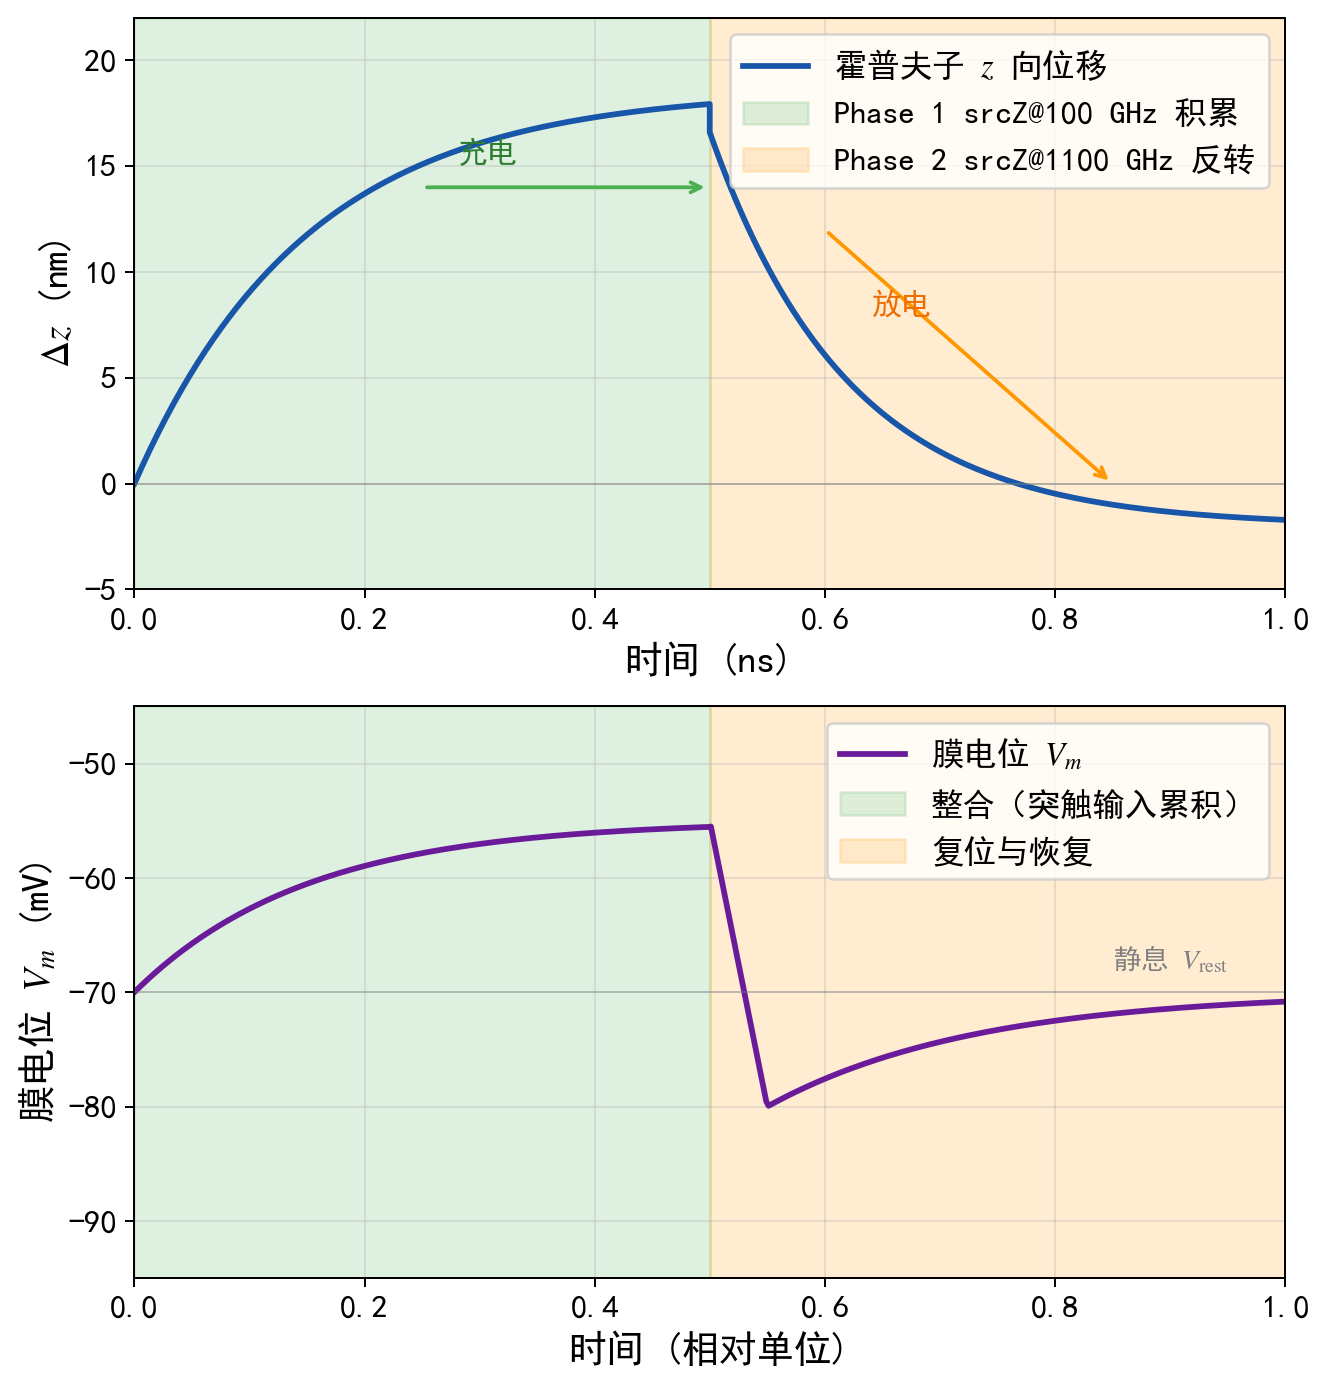
\includegraphics[width=0.75\textwidth]{figures/fig6-1_lif_analogy.png}
  \caption{霍普夫子双向控制位移曲线与 LIF（Leaky Integrate and Fire，泄漏积分发放）神经元膜电位的类比。(a) Phase~1 在 srcZ@\SI{100}{GHz} 激励下位移积累至峰值 $+\SI{18.6}{nm}$，Phase~2 切换至 srcZ@\SI{1100}{GHz} 后位移快速回落，波形呈先积累后释放特征；(b) LIF 神经元膜电位在整合期由静息电位 $V_{\mathrm{rest}}$ 经突触电流累积后进入复位恢复阶段，两者在时序演化模式上形成直接映射。}
  \label{fig:lif-analogy}
\end{figure}

\section{概念器件设计}

基于上述微磁学与神经元功能的映射关系，提出一种以霍普夫子为核心信息载体的自旋波神经形态器件架构，其物理构型如\cref{fig:device-concept}所示。在该逻辑架构中，微波天线阵列作为突触输入端，通过激发特定频率与极化的自旋波将外部电信号耦合至纳米磁轨道。天线在频率、幅度及传播模式上的差异化配置构成了多维突触输入空间。内嵌于磁轨道中的霍普夫子充当神经元胞体，其物理空间位置的变化表征神经元状态的演化，而结构本身的频率响应死区则充当非线性激活阈值。在输出读取端，通过隧道磁阻（TMR）或巨磁阻（GMR）效应将霍普夫子的位置偏移转化为可测量的电压脉冲信号。此外，自旋波驱动幅度与霍普夫子位移速度之间的正相关标度律，提供了实现突触权重连续调节的物理基础。

\begin{figure}[H]
  \centering
  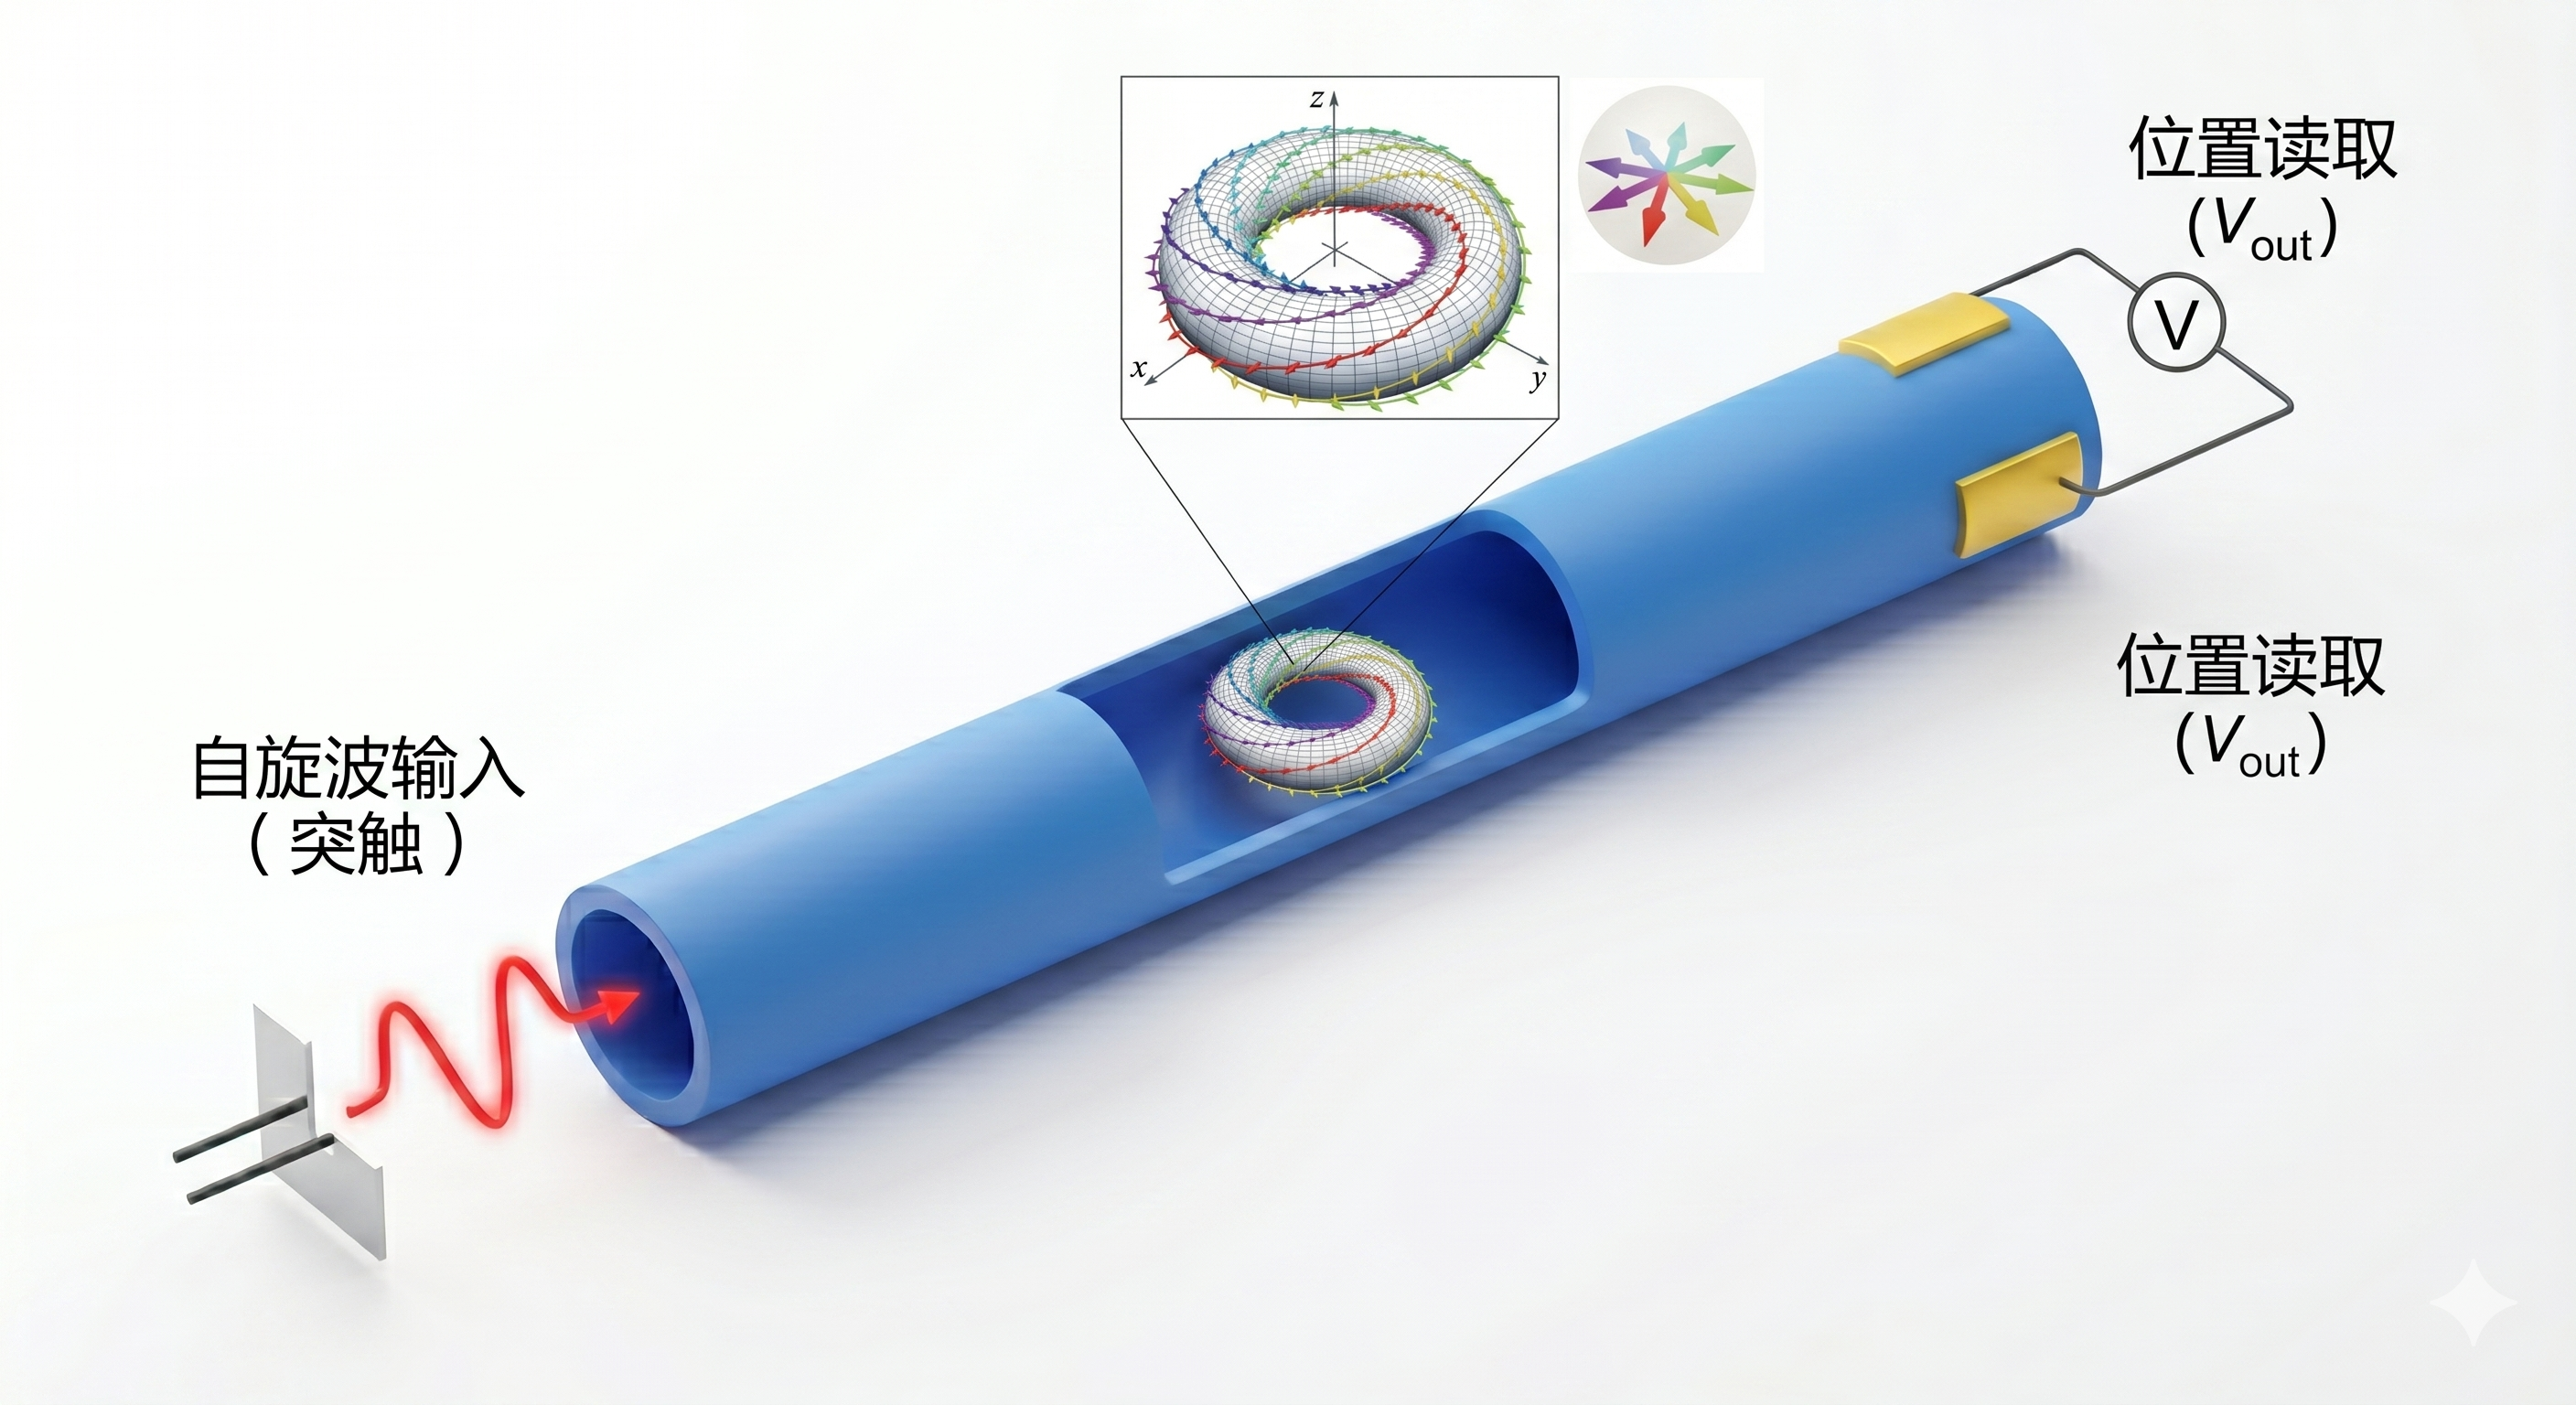
\includegraphics[width=0.8\textwidth]{figures/fig6-2_device_concept.png}
  \caption{霍普夫子自旋波神经形态概念器件示意。左端微波天线作为突触输入端激发自旋波，沿纳米磁轨道传播并驱动内嵌霍普夫子产生轴向位移，右端电极通过磁阻效应读取霍普夫子位置编码的电压信号。顶部放大图展示霍普夫子的三维纽结自旋构型。}
  \label{fig:device-concept}
\end{figure}

相较于基于二维斯格明子的神经形态方案，三维霍普夫子在磁畴存储密度与动力学调控自由度上具备内在优势。其三维拓扑保护机制能够赋予器件更强的抗热涨落能力，而全自旋波驱动架构则从根本上避免了传统电流驱动方案中的高焦耳热功耗问题。

将上述概念架构转化为实际物理器件仍需克服多项工程挑战。当前关于霍普夫子的实验观测多局限于超低温环境\cite{zheng2023hopfion}，室温下稳定承载三维纽结构型的材料体系尚待发掘。同时，阻挫交换体系中霍普夫子的纳米级特征尺寸逼近现有微纳加工技术的极限，且自旋波在受限几何磁轨道中的长距离相干传播机制仍需进一步的实验验证。

本章提取了霍普夫子在自旋波激励下的频率选择性、方向编码以及仿膜电位时序演化等动力学特征。通过建立微磁学行为与 LIF 神经元模型的逻辑映射关系，提出了自旋波神经形态器件的底层架构设计，为三维拓扑磁结构在低功耗类脑计算领域的应用提供了数值理论支撑。
